\documentclass[a1paper,20pt]{tikzposter}
%\usepackage{fixltx2e}
\usepackage{paralist}
\usepackage{tabularx}
\usepackage{IEEEtrantools}
\usepackage{url}
\tikzposterlatexaffectionproofoff

\title{\parbox{\linewidth}{\vspace{0.2em}\centering
A Web-based graphical interface for microscopy image analysis on a GPU cluster\vspace{0.2em}}
}
\author{
Hoang Anh\,Nguyen,
Zane van\,Iperen,
Jake\,Carroll,
Nicholas D\,Condon,
David\,Abramson,
James\,Springfield
}
\institute{
\,The\,University\,of\,Queensland.
}
\titlegraphic{
\includegraphics[height=4cm]{rcc.png}   
\includegraphics[height=4cm]{imb.png}\hfill 

\includegraphics[height=4cm]{uq.png}}

%\usetheme{Default}
\definecolorstyle{uq} {
\definecolor{uq-purple}{HTML}{49075e}
\definecolor{uq-green}{HTML}{8cb800}
\definecolor{uq-gold}{HTML}{bda14e}
%\definecolor{uq-blue}{HTML}{3a7dda}
\definecolor{uq-blue}{HTML}{005ea5}
%\definecolor{uq-aqua}{HTML}{0091b5}
\definecolor{uq-emerald}{HTML}{39892f}
}{
% Background Colors
\colorlet{backgroundcolor}{lightgray}
\colorlet{framecolor}{lightgray}
% Title Colors
\colorlet{titlefgcolor}{white}
\colorlet{titlebgcolor}{uq-purple}
% Block Colors
\colorlet{blocktitlebgcolor}{uq-blue}
\colorlet{blocktitlefgcolor}{white}
\colorlet{blockbodybgcolor}{white}
\colorlet{blockbodyfgcolor}{black}
% Innerblock Colors
\colorlet{innerblocktitlebgcolor}{white}
\colorlet{innerblocktitlefgcolor}{black}
\colorlet{innerblockbodybgcolor}{uq-gold!50!white}
\colorlet{innerblockbodyfgcolor}{black}
% Note colors
\colorlet{notefgcolor}{black}
\colorlet{notebgcolor}{uq-blue!50!white}
\colorlet{noteframecolor}{uq-blue}
}

\usecolorstyle{uq}
\usebackgroundstyle{VerticalGradation}
\usetitlestyle[width=\textwidth,roundedcorners=2,linewidth=1mm,titletotopverticalspace=0mm]{Default}
\useblockstyle[roundedcorners=2,linewidth=1mm,titleinnersep=6mm,bodyinnersep=6mm]{Default}

\begin{document}
\bibliographystyle{IEEEtran}
\bstctlcite{IEEEexample:BSTcontrol}

\maketitle
\begin{columns}
\column{0.34}
\block{Abstract}{
We present a Web portal that is capable of performing large scale, batch processing of microscopy images on a GPU cluster. This portal provides users with user-friendly Web pages to convert between image formats and submit deconvolution jobs. Currently the deconvolution is performed with the microvolution package \cite{microvolution} in the Wiener cluster \cite{wiener}, but the portal can be easily extended to use other tools and run on other clusters. In conjunction with MeDiCI (Metropolitan Data Caching Infrastructure) \cite{datastorage}, we aim to provide a seamless solution that could automatically transfer the images from the acquisition machines to high-performance computing clusters for analysis and archive the results for visualisation or further processing. 
The portal is currently available to UQ users at: https://imbmicroscopy.rcc.uq.edu.au.
}


\block{Motivation}{
\vspace{0.45em}
Microscopic image analysis is a complex process, often involves the coordination of multiple resources, such as instruments, computers and data stores, across multiple logical and physical domains. The whole process is rather complicated for average scientists. 


\vspace{0.45em}
The IMBMicroscopy Web portal, together with MeDICI, streamlines this process so that any scientists could perform microscopy image analysis at scale.  
\vspace{0.45em}
}

\block{Main Features}{
\vspace{0.45em}
\vspace{0.45em}
\begin{compactitem}
  \item Convert between multiple image formats 
  \item Generate PSF files
  \item Deconvolve multiple images in batch-mode using GPU using microvolution package
  \item Manage files and jobs
\end{compactitem}
\vspace{0.45em}
}

%\block{FAQ}{
%\vspace{0.45em}
%\vspace{0.45em}
%\begin{compactitem}
%  \item Who can use the portal  
%  \textit{Anyone with an UQ account that is already in the Wiener GPU cluster.}
%  \item What is it running ?
%  \item Deconvole in batch-mode of multiple images using GPU with microvolution
%\end{compactitem}
%\vspace{0.45em}
%}

\block{}{\small{\textbf{Contact}: \url{h.nguyen30@uq.edu.au}}}
\block[titleinnersep=3mm,bodyinnersep=3mm]{\small References}{
\small \vspace{-1em}
%\bibliographystyle{ieeetr}
\renewcommand{\section}[2]{}
\bibliography{reference}
}


\column{0.66}

\block{}{
\vspace{1em}
\begin{tikzfigure}[IMBMicroscopy Portal]
  \label{fig:portal}
  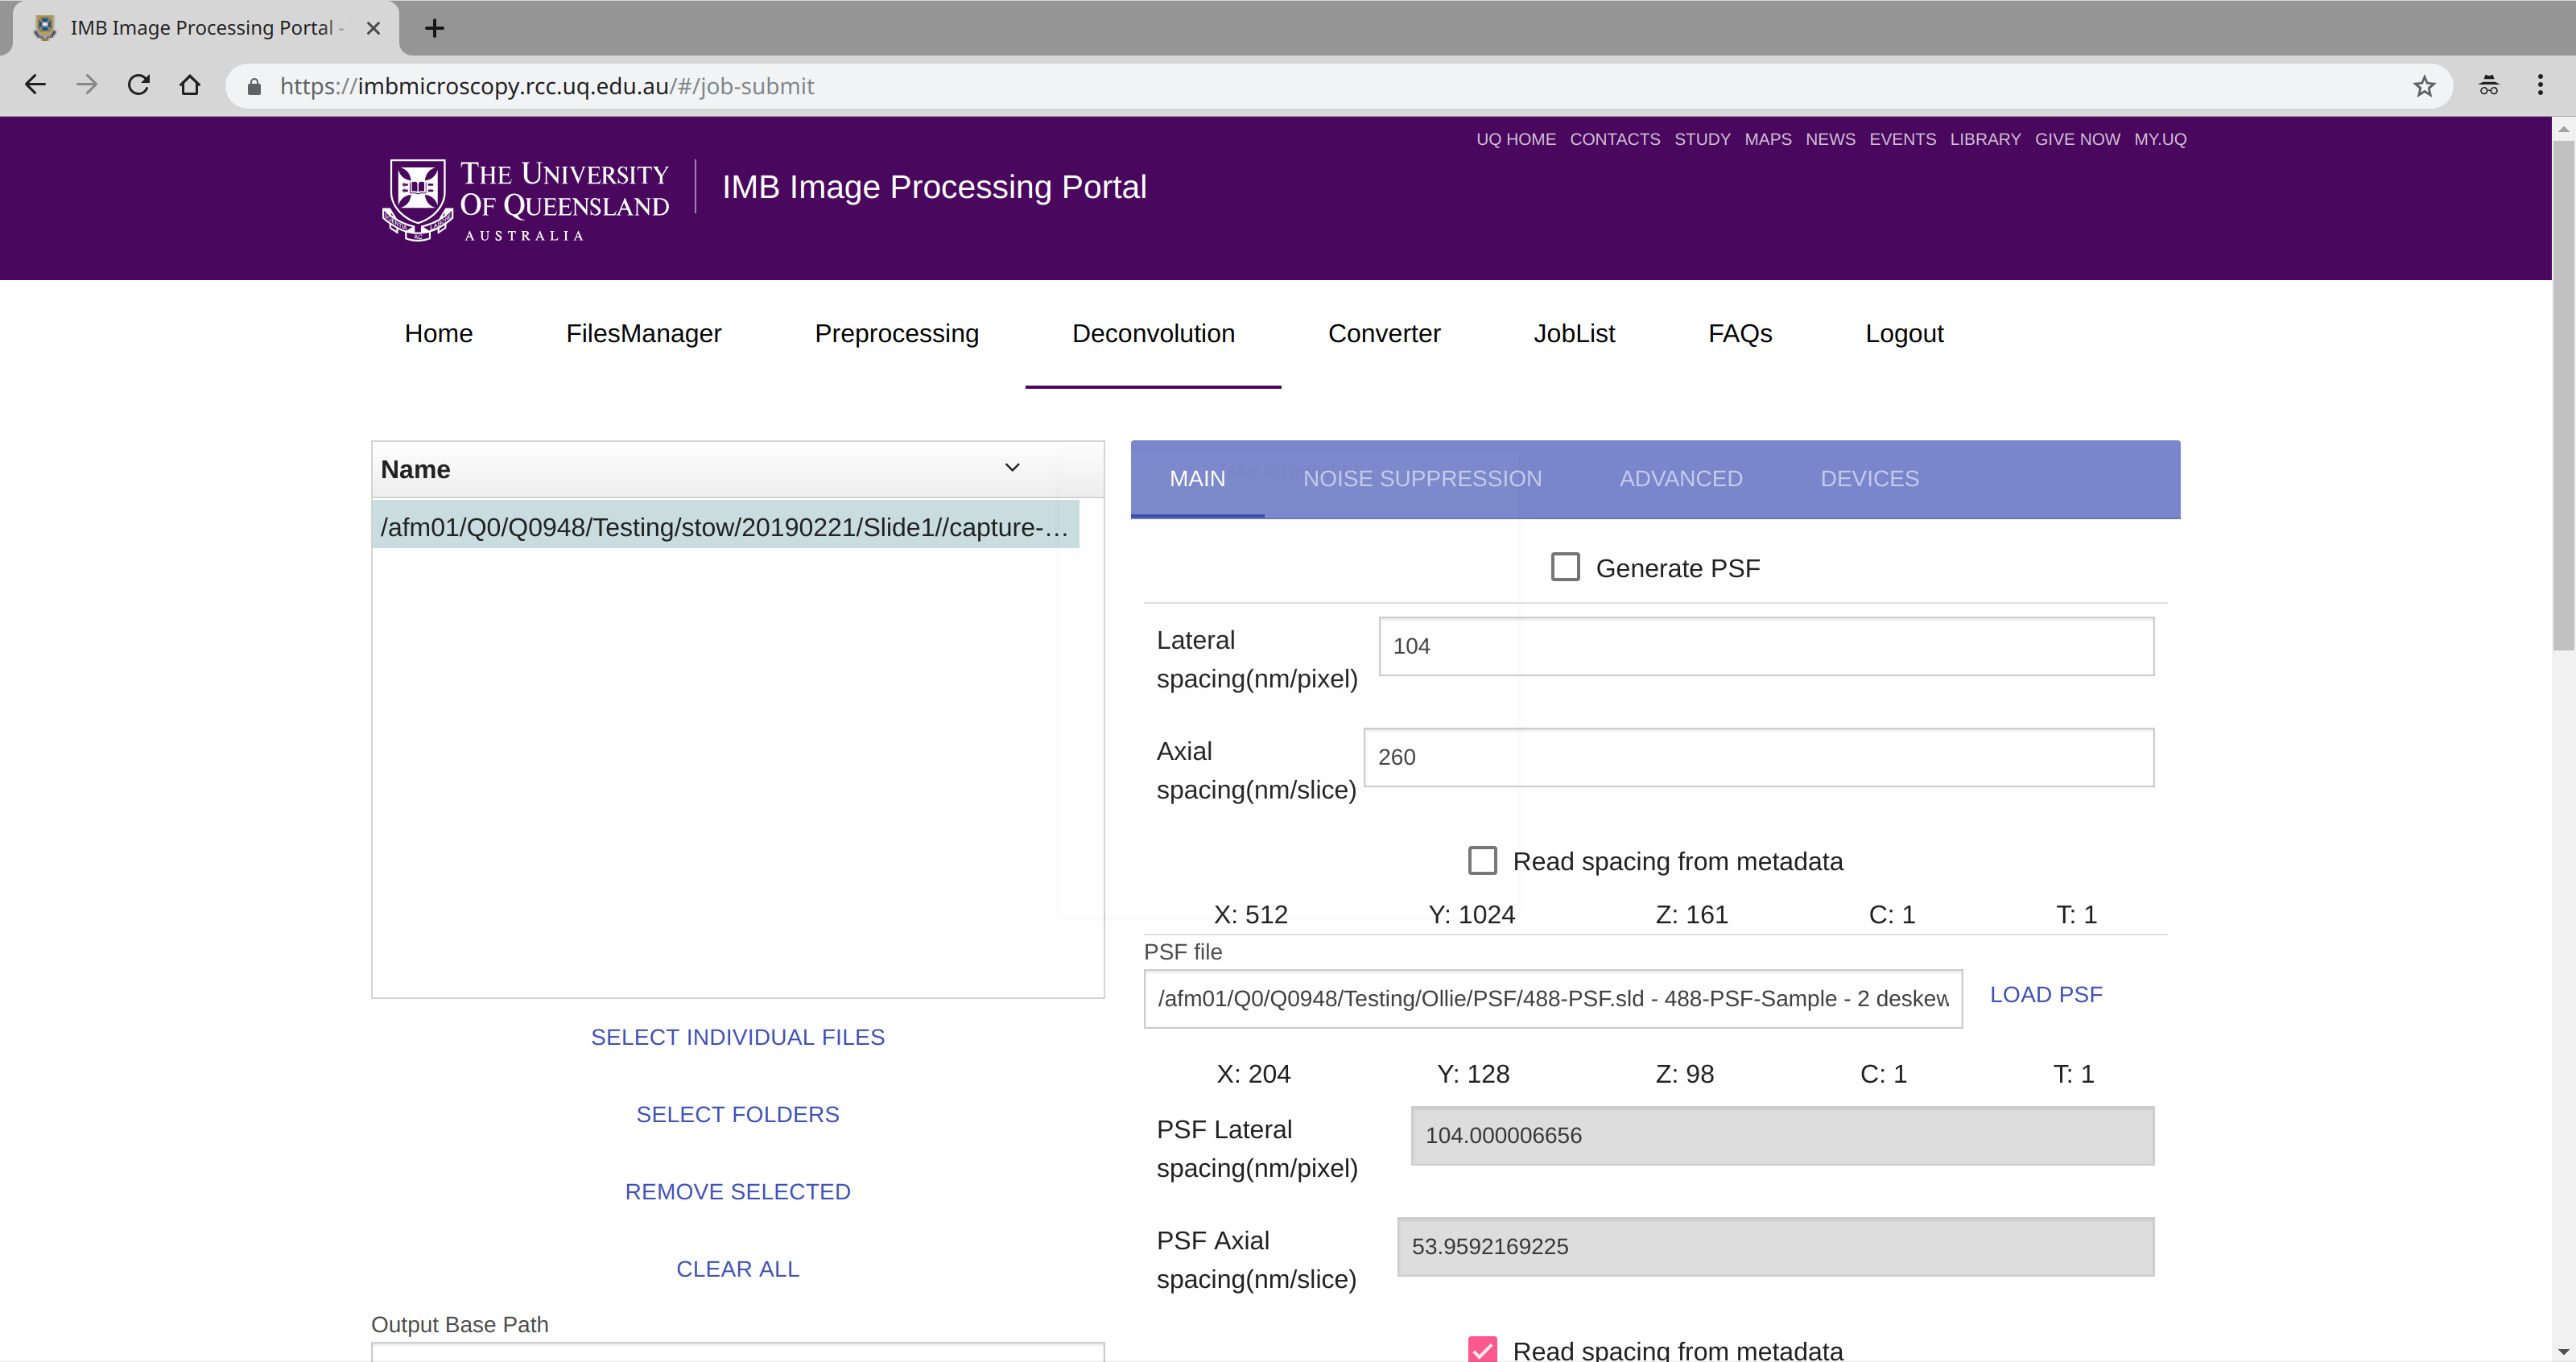
\includegraphics[width=1.0\linewidth]{portal.png}
\end{tikzfigure}
\vspace{0.45em}
}

\block{Image Analysis Workflow}{
Figure~\ref{fig:workflow} shows the image analysis workflow and where the portal fits in the UQ's storage and computation landscape.
\begin{tikzfigure}[Image analysis workflow]
  \label{fig:workflow}
  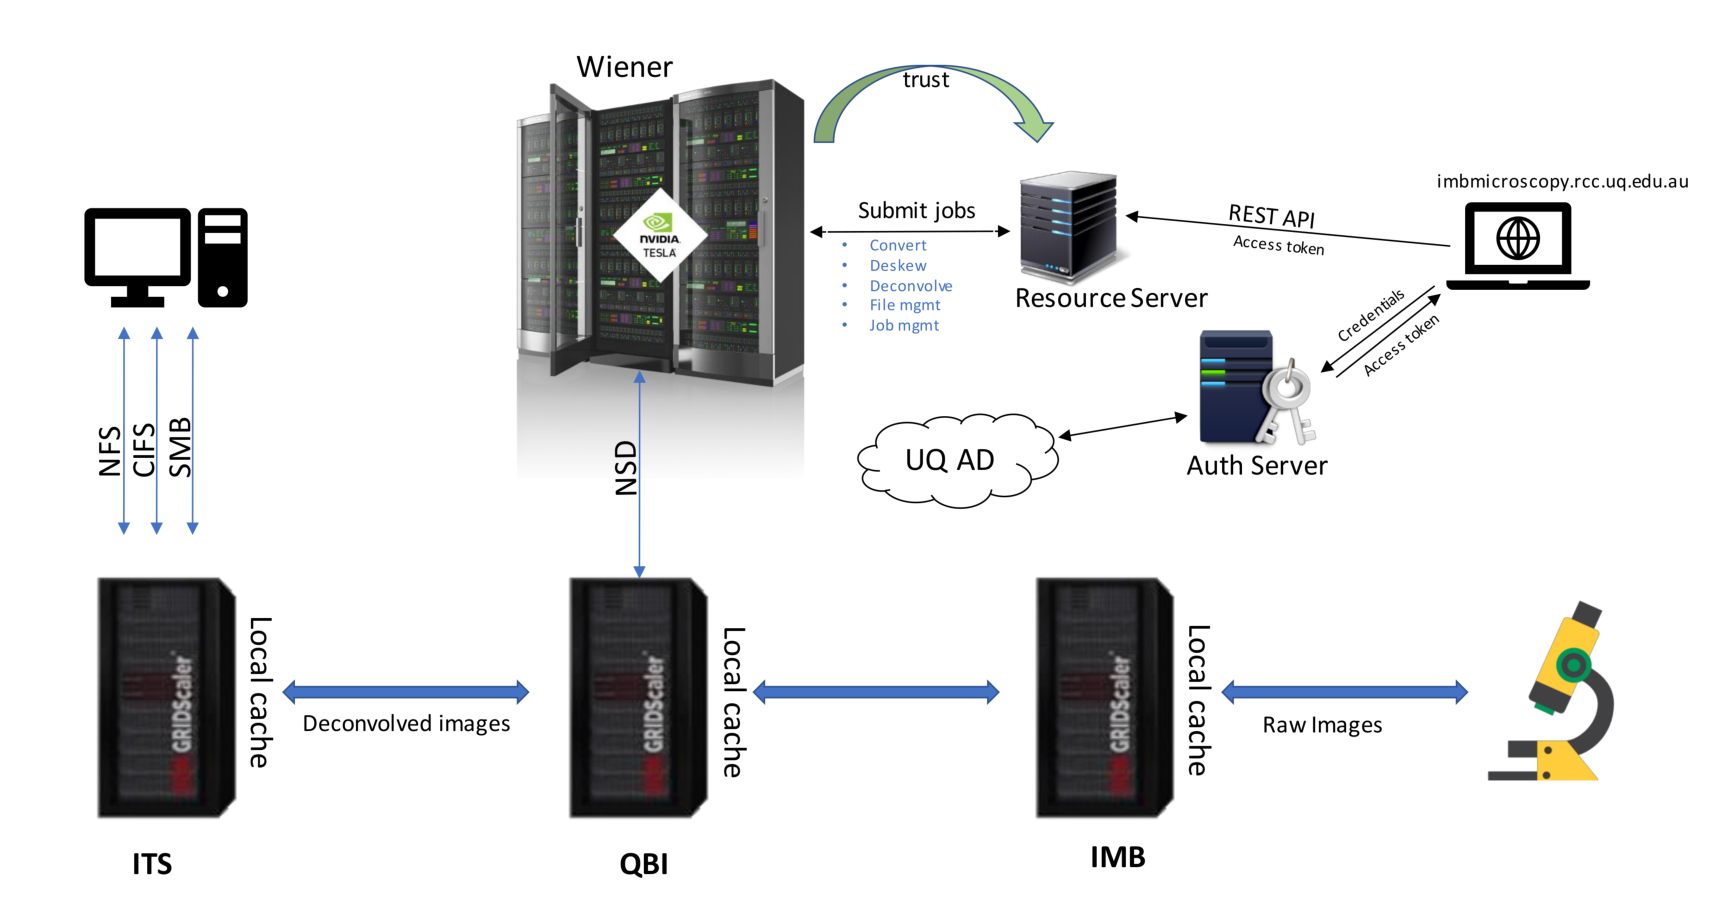
\includegraphics[width=1.0\linewidth]{architecture.pdf}
  \vspace{-2.7em}
\end{tikzfigure}
\vspace{0.45em}
MeDiCI \cite{datastorage} (Metropolitan Data Caching Infrastructure) is a high performance data storage fabric for UQ. It allows data to be automatically transferred for storage and sharing purposes without any manual involvement. UQ users can access their data in a number of ways, i.e. direct mount on workstations and clusters on campus, or sync the data to portable devices such as laptops. 

\vspace{0.45em}
Wiener \cite{wiener} is a GPU (Graphics Processing Units) high-performance cluster in UQ. All the computational jobs created by the portal are performed in Wiener. 
\vspace{0.45em}
}



\end{columns}

\end{document}
